\documentclass[11pt,a4paper]{article}

\usepackage[utf8]{inputenc}
\usepackage[T1]{fontenc}
\usepackage[spanish,es-tabla]{babel}
\usepackage[margin=2.2cm]{geometry}
\usepackage{amsmath,amssymb,amsfonts,amsthm}
\usepackage{booktabs}
\usepackage{tabularx}
\usepackage{array}
\usepackage{graphicx}
\usepackage{placeins}
\usepackage{hyperref}
\hypersetup{
  pdftitle={Material Suplementario: Normalizacion Causal en Factor de Capacidad y Regresor Huber Estructurado (SM-CFHR)},
  pdfauthor={Jesus David Arevalo Montilla; Enmanuel David Diaz Molinares},
  pdfsubject={Material suplementario de SM-CFHR},
  pdfkeywords={SM-CFHR, Lean 4, Newey-West HAC, MCS, SPA, Pronostico fotovoltaico}
}

\newcolumntype{L}{>{\raggedright\arraybackslash}X}
\providecommand{\botrule}{\bottomrule}
\newtheorem{theorem}{Teorema}
\newtheorem{proposition}{Proposición}
\DeclareMathOperator{\clip}{clip}
\DeclareMathOperator{\diag}{diag}
\DeclareMathOperator{\MAD}{MAD}
\DeclareMathOperator{\sign}{sign}

\newcounter{algoritmo}
\renewcommand{\thesection}{S\arabic{section}}
\renewcommand{\thetable}{S\arabic{table}}
\renewcommand{\thefigure}{S\arabic{figure}}
\renewcommand{\theequation}{S\arabic{equation}}
\renewcommand{\thealgoritmo}{S\arabic{algoritmo}}

\begin{document}

\begin{center}
{\Large\bfseries Material Suplementario: Normalización Causal en Factor de Capacidad y Regresor Huber Estructurado (SM-CFHR)}\\[0.6em]
{\normalsize Jesús David Arévalo Montilla y Enmanuel David Diaz Molinares}\\
{\small Departamento de Matemáticas y Ciencia de Datos, Universidad del Norte, Barranquilla, Colombia}
\end{center}

\vspace{0.5em}
\hrule
\vspace{1em}

\section{Demostraciones matemáticas completas, estructura diferencial y complejidad}\label{sup:demos}

Esta sección reúne las demostraciones completas de los resultados analíticos resumidos en el manuscrito principal, distinguiendo expresamente las aplicaciones directas de la teoría convexa y robusta clásica \cite{boyd2004convex,huber1964,hampel1986robust,huber2009robust} de las verificaciones específicas para SM-CFHR.

Considérese el programa convexo en espacio estandarizado ($\tilde{y}_k = (y_k - m_y)/\sigma_y$ con $\sigma_y > 0$, $\mathbf{z}_k \in \mathbb{R}^p$, $D_\alpha = \diag(d_1,\dots,d_p)$ con $d_j \in \{\alpha_{\mathrm{lin}}, \alpha_{\mathrm{meteo}}\}$):
\begin{equation}
\min_{b \in \mathbb{R},\; \mathbf{w} \in \mathcal{C}} \; J(b, \mathbf{w}) := \frac{1}{n}\sum_{k=1}^{n} \rho_\delta\!\left(\tilde{y}_k - b - \mathbf{z}_k^\top \mathbf{w}\right) + \frac{1}{2}\mathbf{w}^\top D_\alpha \mathbf{w},
\label{eq:sup_obj}
\end{equation}
donde $\mathcal{C} = \{\mathbf{w} \in \mathbb{R}^p : w_j \ge 0 \;\forall j \in \mathcal{M}_+\}$, $\Omega = \mathbb{R} \times \mathcal{C}$, y la derivada de Huber es $\psi_\delta(r) = \clip(r, -\delta, \delta)$.

\begin{theorem}[Convexidad, regularidad $C^1$, coercividad y existencia]\label{sup:thm_conv}
Si $n \ge 1$, $\delta > 0$ y $\alpha_{\mathrm{lin}}, \alpha_{\mathrm{meteo}} > 0$, entonces: (1) $\Omega$ es cerrado y convexo; (2) $J \in C^1(\mathbb{R}^{p+1})$ es convexa y $\nabla J$ es globalmente Lipschitz con constante $L_J \le \frac{1}{n}\left\|\begin{bmatrix}\mathbf{1}_n & Z\end{bmatrix}\right\|_2^2 + \max\{\alpha_{\mathrm{lin}}, \alpha_{\mathrm{meteo}}\}$; y (3) $J$ es coerciva sobre $\Omega$ y admite al menos un minimizador global $(b^*, \mathbf{w}^*) \in \Omega$.
\end{theorem}

\begin{proof}
\textbf{(1)} $\Omega = \mathbb{R} \times \mathcal{C}$ es producto cartesiano de $\mathbb{R}$ y el poliedro $\mathcal{C} = \bigcap_{j \in \mathcal{M}_+} \{\mathbf{w} \in \mathbb{R}^p : w_j \ge 0\}$, intersección de semiespacios cerrados y convexos en $\mathbb{R}^p$ \cite{boyd2004convex}.

\textbf{(2)} La función de Huber $\rho_\delta$ es de clase $C^1(\mathbb{R})$ con derivada $1$-Lipschitz $\psi_\delta$ \cite{huber1964}. Sea $A := \begin{bmatrix} \mathbf{1}_n & Z \end{bmatrix} \in \mathbb{R}^{n \times (p+1)}$ y $\boldsymbol{\theta} := (b, \mathbf{w}) \in \mathbb{R}^{p+1}$. Por composición afín y suma con $\frac{1}{2}\mathbf{w}^\top D_\alpha \mathbf{w}$ ($D_\alpha \succ 0$), $J \in C^1(\mathbb{R}^{p+1})$ es convexa. Para $\boldsymbol{\theta}_1, \boldsymbol{\theta}_2 \in \mathbb{R}^{p+1}$ con $\mathbf{r}_1 = \tilde{\mathbf{y}} - A\boldsymbol{\theta}_1$ y $\mathbf{r}_2 = \tilde{\mathbf{y}} - A\boldsymbol{\theta}_2$:
\begin{align*}
\|\nabla J(\boldsymbol{\theta}_1) - \nabla J(\boldsymbol{\theta}_2)\|_2
&\le \frac{1}{n}\|A^\top (\psi_\delta(\mathbf{r}_2) - \psi_\delta(\mathbf{r}_1))\|_2 + \|D_\alpha(\mathbf{w}_1 - \mathbf{w}_2)\|_2 \\
&\le \left(\frac{1}{n}\|A\|_2^2 + \max\{\alpha_{\mathrm{lin}}, \alpha_{\mathrm{meteo}}\}\right)\|\boldsymbol{\theta}_1 - \boldsymbol{\theta}_2\|_2.
\end{align*}

\textbf{(3)} Como $J(b,\mathbf{w}) \ge 0$, fijado $C \in \mathbb{R}$ arbitrario defínanse $C_+ := \max\{C, 0\} + 1$, $\alpha_{\min} := \min\{\alpha_{\mathrm{lin}}, \alpha_{\mathrm{meteo}}\} > 0$,
\[
R_w := \sqrt{\frac{2 C_+}{\alpha_{\min}}} + 1, \qquad
R_b := \|\tilde{\mathbf{y}}\|_\infty + \|Z\|_{\infty,2}\,R_w + n\left(\frac{C_+}{\delta} + \frac{\delta}{2}\right) + 1,
\]
y $R := \max\{R_w, R_b\}$. Para todo $(b, \mathbf{w}) \in \Omega$ con $\|(b, \mathbf{w})\|_2 > \sqrt{2}\,R$: si $\|\mathbf{w}\|_2 > R_w$, entonces $\frac{1}{2}\mathbf{w}^\top D_\alpha \mathbf{w} > C_+ > C$; si $\|\mathbf{w}\|_2 \le R_w$, entonces $|b| > R_b$, de modo que para cualquier índice $k \in \{1,\dots,n\}$ se cumple $|r_k| \ge |b| - \|\tilde{\mathbf{y}}\|_\infty - \|Z\|_{\infty,2} R_w > n(C_+/\delta + \delta/2)$ y, usando $\rho_\delta(r) \ge \delta(|r| - \delta/2)$, resulta $J(b, \mathbf{w}) \ge \frac{\delta}{n}(|r_k| - \delta/2) > C_+ > C$. Al ser $J$ continua, acotada inferiormente y coerciva sobre el cerrado $\Omega$, el teorema de Weierstrass garantiza la existencia de un minimizador global.
\end{proof}

\begin{theorem}[Unicidad de pesos y unicidad condicional del intercepto]\label{sup:thm_unic}
Bajo las hipótesis del Teorema~\ref{sup:thm_conv}: (1) el vector $\mathbf{w}^*$ es único; (2) si existe $(b^*, \mathbf{w}^*)$ y algún $k$ con $|\tilde{y}_k - b^* - \mathbf{z}_k^\top \mathbf{w}^*| < \delta$, entonces $b^*$ es único; y (3) si todos los residuos óptimos satisfacen $|r_k^*| \ge \delta$, el intercepto puede no ser único.
\end{theorem}

\begin{proof}
\textbf{(1)} Si $(b_1, \mathbf{w}_1), (b_2, \mathbf{w}_2) \in \Omega$ fuesen óptimos con $\mathbf{w}_1 \ne \mathbf{w}_2$, el punto medio $\bar{\boldsymbol{\theta}} \in \Omega$ tendría menor valor objetivo por estricta convexidad de $\frac{1}{2}\mathbf{w}^\top D_\alpha \mathbf{w}$ ($D_\alpha \succ 0$), contradicción.

\textbf{(2)} Fijado $\mathbf{w}^*$, $g(b) := J(b, \mathbf{w}^*)$ es convexa, continua y coerciva, luego su conjunto de mínimos es un intervalo compacto $[b_{\min}, b_{\max}]$. Si $b_{\min} < b_{\max}$ y existiese $k$ con $|r_k(b^*)| < \delta$, por continuidad existiría un subintervalo abierto $(u,v) \subset [b_{\min}, b_{\max}]$ donde $|r_k(b)| < \delta$ y el término cuadrático $\frac{1}{2n}(c_k - b)^2$ haría a $g$ estrictamente convexa en $(u,v)$, contradiciendo que $g$ sea constante en $[b_{\min}, b_{\max}]$.

\textbf{(3)} Con $n=2$, $Z = \mathbf{0}$ y $\tilde{\mathbf{y}} = (-2\delta, +2\delta)^\top$, $\mathbf{w}^* = \mathbf{0}$ y para todo $b \in [-\delta, \delta]$ ambos residuos cumplen $|\pm 2\delta - b| \ge \delta$, resultando $g(b) = \frac{3}{2}\delta^2$ constante.
\end{proof}

\begin{proposition}[Condiciones KKT, influencia y monotonía]\label{sup:prop_kkt}
Un punto $(b^*, \mathbf{w}^*) \in \Omega$ es óptimo global de \eqref{eq:sup_obj} si y solo si existen $\lambda_j^* \ge 0$ ($j \in \mathcal{M}_+$) tales que:
\[
-\frac{1}{n}\sum_{k=1}^n \psi_\delta(r_k^*) = 0, \quad
-\frac{1}{n}(Z^\top \psi_\delta(\mathbf{r}^*))_j + d_j w_j^* = \begin{cases} \lambda_j^* \text{ con } \lambda_j^* w_j^* = 0 & j \in \mathcal{M}_+, \\ 0 & j \notin \mathcal{M}_+. \end{cases}
\]
Además, cada observación satisface $\left|\frac{1}{n}\psi_\delta(r_k^*)\right| \le \frac{\delta}{n}$ y $\left\|\frac{1}{n}\mathbf{z}_k \psi_\delta(r_k^*)\right\|_\infty \le \frac{\delta}{n}\|\mathbf{z}_k\|_\infty$ (acotada en respuesta, lineal en apalancamiento $\mathbf{z}_k$), y la predicción truncada $\hat{y}_q = \clip(m_y + \sigma_y(\hat{b} + \mathbf{z}_q^\top \hat{\mathbf{w}}), 0, 1)\cdot 24\,000\,C_{i,t} H_{\mathrm{dir}}$ es no decreciente en cada coordenada $j \in \mathcal{M}_+$ con $\tilde{s}_j > 0$.
\end{proposition}

\begin{proof}
Las restricciones $-w_j \le 0$ ($j \in \mathcal{M}_+$) son afines y cumplen Slater ($w_j > 0$), por lo que las condiciones KKT del Lagrangiano $\mathcal{L}(b,\mathbf{w},\boldsymbol{\lambda}) = J(b,\mathbf{w}) - \sum_{j \in \mathcal{M}_+} \lambda_j w_j$ son necesarias y suficientes \cite{boyd2004convex}. La cota en el gradiente se sigue directamente de $|\psi_\delta(r)| \le \delta$, y la monotonía parcial se sigue de $z_{q,j}' - z_{q,j} = \Delta/\tilde{s}_j > 0$, $w_j^* \ge 0$, $\sigma_y > 0$ y la monotonía de $\clip(\cdot, 0, 1)$.
\end{proof}

\subsection{Estructura diferencial por tramos y complejidad computacional}

Aunque $J \in C^1(\mathbb{R}^{p+1})$ tiene gradiente Lipschitz continuo, no es de clase $C^2$ sobre los hiperplanos de transición $|r_k(b,\mathbf{w})| = \delta$. En el interior de cada región abierta donde $|r_k| \ne \delta$ para todo $k$, la matriz Hessiana existe y toma la forma:
\begin{equation}
\nabla^2 J(b,\mathbf{w}) = \frac{1}{n} \begin{bmatrix} \mathbf{1}_n^\top \\ Z^\top \end{bmatrix} \diag(\mathbf{1}_{\mathcal{I}_{\mathrm{quad}}}) \begin{bmatrix} \mathbf{1}_n & Z \end{bmatrix} + \begin{bmatrix} 0 & \mathbf{0}^\top \\ \mathbf{0} & D_\alpha \end{bmatrix},
\label{eq:sup_hessiana}
\end{equation}
donde $\mathcal{I}_{\mathrm{quad}} := \{k \in \{1,\dots,n\} : |r_k| < \delta\}$ agrupa las observaciones en régimen cuadrático. Fuera de esos hiperplanos, $\nabla^2 J$ es semidefinida positiva; en los quiebres $|r_k| = \delta$, la segunda derivada presenta saltos finitos, lo que motiva resolver el problema mediante L-BFGS-B de primer orden con proyecciones simples sobre las cotas de caja $\mathbb{R} \times \mathcal{C}$ \cite{byrd1995lbfgsb,zhu1997lbfgsb}.

En términos de complejidad, cada evaluación de $J$ y $\nabla J$ requiere dos productos matriz-vector con $Z \in \mathbb{R}^{n \times p}$ ($O(np)$ operaciones, con $p \in \{7,17\}$). Para un ajuste completo con $K$ iteraciones de L-BFGS-B ($m=10$ pares de curvatura en memoria), el coste es $O(np + Knp)$ en tiempo y $O(np + mp)$ en memoria tras el preprocesamiento inicial $O(np)$. Con búsqueda bayesiana anidada de $B=25$ ensayos TPE sobre $K_{\mathrm{cv}}=3$ particiones internas, el coste escala como $O(B \cdot K_{\mathrm{cv}} \cdot Knp)$, mientras que el despliegue recursivo de horizonte $H$ añade $O(Hp)$ operaciones por origen.

\section{Verificación formal en Lean~4}\label{sup:lean4}

La formalización matemática de SM-CFHR se desarrolló en \textbf{Lean~4} (\texttt{leanprover/lean4:v4.36.0}) \cite{moura2021lean4} sobre \textbf{Mathlib} (revisión \texttt{fc4f59e577feb1a4956671bc04ac18aaaf8cd842}) \cite{mathlib2020}, compilando $26$ declaraciones sin axiomas personalizados (únicamente \texttt{propext}, \texttt{Classical.choice} y \texttt{Quot.sound}), resumidas en la Tabla~\ref{tab:sup_lean4}. Para reproducir la verificación en un entorno Lean~4 (\texttt{v4.36.0}) con acceso a la caché de Mathlib, ejecútese \texttt{lake exe cache get \&\& lake build \&\& lake env lean SMCFHR/AxiomsAudit.lean} dentro de \texttt{formal/sm\_cfhr\_lean/}.

\begin{table}[!htbp]
\centering
\caption{Correspondencia entre enunciados matemáticos y declaraciones compiladas en Lean~4 (\texttt{v4.36.0}).}
\label{tab:sup_lean4}
\scriptsize
\begin{tabularx}{\textwidth}{@{}p{3.0cm}p{3.2cm}L@{}}
\toprule
Resultado & Módulo Lean~4 & Declaraciones compiladas (26 en total) \\
\midrule
Proyección física $[0,1]$ & \texttt{Clipping.lean}, \texttt{Monotonicity.lean} & \texttt{clip01\_nonneg}, \texttt{clip01\_le\_one}, \texttt{clip01\_mono}, \texttt{predictCF\_bounds}, \texttt{predictEnergy\_bounds} \\
Pérdida de Huber & \texttt{Huber.lean} & \texttt{huber\_nonneg}, \texttt{psi\_abs\_le}, \texttt{psi\_lipschitz}, \texttt{hasDerivAt\_huber}, \texttt{convexOn\_huber}, \texttt{strictConvexOn\_huber\_band} \\
Teorema~\ref{sup:thm_conv}(1)--(2) & \texttt{Model.lean}, \texttt{Gradient.lean} & \texttt{convex\_feasibleSet}, \texttt{isClosed\_feasibleSet}, \texttt{convexOn\_objective}, \texttt{hasDerivAt\_objective\_line}, \texttt{objective\_subgradient}, \texttt{gradB\_lipschitz} ($\partial J/\partial b$; la cota espectral completa $L_J$ de $\nabla J$ figura en la Sección~\ref{sup:demos}) \\
Teorema~\ref{sup:thm_conv}(3) & \texttt{Optimality.lean} & \texttt{objective\_coercive}, \texttt{exists\_global\_minimizer} \\
Teorema~\ref{sup:thm_unic}(1)--(3) & \texttt{Optimality.lean} & \texttt{unique\_weights}, \texttt{unique\_intercept\_of\_interior\_residual}, \texttt{intercept\_nonunique\_counterexample} \\
Proposición~\ref{sup:prop_kkt} & \texttt{Optimality.lean}, \texttt{Gradient.lean}, \texttt{Monotonicity.lean} & \texttt{kkt\_iff\_isMinOn}, \texttt{gradB\_term\_bound}, \texttt{gradW\_term\_bound}, \texttt{predictEnergy\_monotone\_in\_restricted} \\
\bottomrule
\end{tabularx}
\end{table}

\section{Inventarios completos, parámetros operativos y despliegue recursivo}\label{sup:tablas}

\section{Especificaciones de notación, características, escenarios y benchmarks}\label{ap:escenarios}

La Tabla~\ref{tab:notacion} resume los símbolos principales del artículo. La Tabla~\ref{tab:features17} inventaría las $17$ características causales producidas por \texttt{extract\_cf\_features}, indicando su grupo de regularización y si están sujetas a restricción de monotonía no negativa. La Tabla~\ref{tab:config_fixed_hpo} compara las variantes \texttt{SM-CFHR-Fixed} y \texttt{SM-CFHR-HPO}, la Tabla~\ref{tab:escenarios28} enumera los $28$ escenarios oficiales y la Tabla~\ref{tab:benchmarks22} detalla los $22$ procedimientos de referencia.

\begin{table}[!htbp]
\caption{Glosario de notación matemática.}\label{tab:notacion}
\scriptsize
\begin{tabular}{@{}lp{9.5cm}@{}}
\toprule
Símbolo & Significado y unidades \\
\midrule
$M, G$ & Número de plantas ($M=17$) y grupos espaciales ($G=7$) \\
$C_{i,s}, y_{i,s}$ & Capacidad efectiva neta (MW) y generación diaria observada (kWh/día) \\
$E^{\max}_{i,t}$ & Energía nominal máxima diaria al origen: $24\,000\,C_{i,t}$ (kWh/día) \\
$H, H_{\mathrm{dir}}$ & Horizonte en días ($1,7,14,21,28$) y factor de escala directo ($1$ o $H$) \\
$\gamma_h$ & Factor de amortiguamiento geométrico en paso $h$: $0{,}85^{h-1}$ \\
$m_y, \sigma_y$ & Mediana y escala robusta MAD ($1{,}4826\,\MAD$) del objetivo en entrenamiento \\
$\delta, \alpha_{\mathrm{lin}}, \alpha_{\mathrm{meteo}}$ & Umbral de Huber y pesos $L_2$ para dinámica/calendario y meteorología \\
$D_\alpha, \mathcal{M}_+$ & Matriz diagonal de penalización e índices con restricción $w_j \ge 0$ \\
$\mathrm{MAE}_{\mathrm{macro}}$ & Error absoluto medio macro promediado por planta (kWh/día o kWh totales) \\
\bottomrule
\end{tabular}
\end{table}

\begin{table}[!htbp]
\caption{Inventario de características causales de SM-CFHR ($p=7$ sin clima; $p=17$ con clima).}\label{tab:features17}
\scriptsize
\begin{tabular}{@{}cllcc@{}}
\toprule
Índice & Variable en código & Definición & Familia $L_2$ & Monotonía \\
\midrule
1--4 & \texttt{month\_sin/cos}, \texttt{doy\_sin/cos} & Armónicos anuales de calendario al objetivo & $\alpha_{\mathrm{lin}}$ & Libre \\
5 & \texttt{cf30} & Factor de capacidad medio móvil 30d al origen & $\alpha_{\mathrm{lin}}$ & $w_5 \ge 0$ \\
6 & \texttt{diff\_7\_30} & $(\mathrm{cf}_7 - \mathrm{cf}_{30}) \cdot 0{,}85^{h-1}$ & $\alpha_{\mathrm{lin}}$ & Libre \\
7 & \texttt{diff\_1\_7} & $(\mathrm{cf}_1 - \mathrm{cf}_7) \cdot 0{,}85^{h-1}$ & $\alpha_{\mathrm{lin}}$ & Libre \\
8 & \texttt{rad\_pron} & Irradiación horizontal pronosticada (NWP) & $\alpha_{\mathrm{meteo}}$ & $w_8 \ge 0$ \\
9--12 & \texttt{temp/nube/humedad/viento\_pron} & Resto de variables meteorológicas pronosticadas & $\alpha_{\mathrm{meteo}}$ & Libre \\
13--17 & \texttt{anom\_*} & Anomalía causal respecto a media móvil 30d ($\le t_0$) & $\alpha_{\mathrm{meteo}}$ & Libre \\
\bottomrule
\end{tabular}
\end{table}

\begin{table}[!htbp]
\caption{Comparación de configuración entre \texttt{SM-CFHR-Fixed} y \texttt{SM-CFHR-HPO}.}\label{tab:config_fixed_hpo}
\scriptsize
\setlength{\tabcolsep}{3pt}
\begin{tabular}{@{}p{2.3cm}p{4.3cm}p{4.8cm}@{}}
\toprule
Componente & \texttt{SM-CFHR-Fixed} (Primaria) & \texttt{SM-CFHR-HPO} (Secundaria) \\
\midrule
Estructura fija & \multicolumn{2}{p{9.2cm}}{\texttt{n\_knots=0}, \texttt{max\_interactions=0}, \texttt{anchor="none"}, \texttt{structured=True}, \texttt{use\_mono=True}} \\
$\delta$ & $1{,}35$ & TPE en $[0{,}5,\; 3{,}0]$ \\
$\alpha_{\mathrm{lin}}$ & $0{,}01$ & TPE log-uniforme en $[10^{-4},\; 1{,}0]$ \\
$\alpha_{\mathrm{meteo}}$ & $0{,}10$ (clima) / $0{,}01$ (sin clima) & TPE log-uniforme en $[10^{-3},\; 10{,}0]$ (clima) \\
Presupuesto HPO & $B = 0$ evaluaciones & $B = 25$ trials Optuna TPE (3 pliegues, embargo 30d) \\
Optimizador & \multicolumn{2}{p{9.2cm}}{L-BFGS-B (\texttt{max\_iter=400}, \texttt{tol=1e-7}, semilla \texttt{2026})} \\
\bottomrule
\end{tabular}
\end{table}

\begin{table}[!htbp]
\caption{Resumen de las $4$ familias y $28$ escenarios oficiales en \texttt{SCENARIOS\_28}.}\label{tab:escenarios28}
\scriptsize
\begin{tabular}{@{}llccc@{}}
\toprule
Familia & Regímenes & Horizontes $H$ & Clima & $N_{\text{esc}}$ \\
\midrule
$D+1$ (\texttt{d1}) & ET, IP & $1$ día & Con / Sin pronóstico $24\text{ h}$ & $4$ \\
Recursivo sin clima (\texttt{recursive}) & ET, IP & $7, 14, 21, 28$ días & Sin meteorología & $8$ \\
Directo sin clima (\texttt{direct}) & ET, IP & $7, 14, 21, 28$ días & Sin meteorología (acumulado) & $8$ \\
Recursivo + GEFSv12 (\texttt{recursive}) & ET, IP & $7, 14, 21, 28$ días & NOAA GEFSv12 (\texttt{00 UTC}) & $8$ \\
\bottomrule
\end{tabular}
\end{table}

\begin{table}[!htbp]
\caption{Inventario oficial de los $22$ modelos de referencia (excluyendo \texttt{CF-BRH}).}\label{tab:benchmarks22}
\scriptsize
\begin{tabular}{@{}lp{9.2cm}@{}}
\toprule
Categoría & Modelos incluidos \\
\midrule
Bibliotecas ($9$) & \texttt{XGBoost} \cite{chen2016}, \texttt{Random Forest} \cite{breiman2001}, \texttt{Ridge} \cite{hoerl1970}, \texttt{SVR} \cite{drucker1997svr}, \texttt{HistGradientBoosting} \cite{friedman2001gbm}, \texttt{k-NN} \cite{cover1967nearest}, \texttt{Lasso} \cite{tibshirani1996}, \texttt{BayesianRidge} \cite{mackay1992}, \texttt{DecisionTree} \cite{breiman1984cart} \\
Personalizados ($12$) & \texttt{RLAC}, \texttt{IWLAR} \cite{cleveland1979robust,atkeson1997locally}, \texttt{WCFC} \cite{bates1969combination,nikodinoska2022elastic}, \texttt{ABGPR} \cite{rasmussen2006gpml}, \texttt{HARC} \cite{laird1982random,bates2015lme4}, \texttt{SRMOS} \cite{glahn1972mos}, \texttt{ELAC} \cite{brown1959statistical}, \texttt{KLAC} \cite{kalman1960approach,harvey1989forecasting}, \texttt{RARC} \cite{huber1964}, \texttt{RQRF} \cite{koenker1978quantiles,meinshausen2006}, \texttt{PDEC} \cite{hyndman2021fpp3}, \texttt{MARB} \\
Referencia base ($1$) & \texttt{Media móvil de 30 días} (\texttt{MM30}) \\
\bottomrule
\end{tabular}
\end{table}


\subsection{Parámetros operativos secundarios y algoritmo de despliegue recursivo}\label{sup:operativos}

El protocolo de preprocesamiento y validación interna incorpora los siguientes resguardos numéricos secundarios: (1) en la imputación de predictores, si una columna completa es no finita en entrenamiento, la mediana se fija en $0$; (2) en la estandarización de predictores, toda columna constante con desviación estándar $s_j \le 10^{-8}$ adopta escala efectiva $\tilde{s}_j = 1$; (3) en el escalado robusto de la respuesta, tanto el estimador $1{,}4826\,\MAD(\mathbf{y})$ como su respaldo mediante desviación estándar poblacional aplican un piso numérico de $10^{-6}$; (4) durante los primeros días de operación sin ventana completa de $30$ días se aplican respaldos jerárquicos causales ($\mathrm{cf}_{30} \leftarrow 0{,}15$, $\mathrm{cf}_7 \leftarrow \mathrm{cf}_{30}$, $\mathrm{cf}_1 \leftarrow \mathrm{cf}_7$); y (5) la búsqueda interna \texttt{SM-CFHR-HPO} descarta particiones que incumplan los tamaños mínimos $n_{\mathrm{tr}} \ge 15$ y $n_{\mathrm{va}} \ge 5$.

En los escenarios recursivos ($H \in \{7,14,21,28\}$), tanto la validación interna de hiperparámetros como la evaluación externa ejecutan el procedimiento causal exacto formalizado en el Algoritmo~\ref{alg:sup_rollout}.

\begin{figure}[!htbp]
\centering
\fbox{\begin{minipage}{0.95\textwidth}
\small
\refstepcounter{algoritmo}\label{alg:sup_rollout}\textbf{Algoritmo~\thealgoritmo: Despliegue recursivo causal exacto desde el origen $t_0$ ($\text{horizonte } H$)}
\begin{enumerate}
    \item \textbf{Inicialización al origen $t_0$:} fijar la capacidad constante al origen $C_{i,t_0}$, la cota energética $E^{\max}_{i,t_0} = 24\,000\,C_{i,t_0}$, la línea base climática de $30$ días $\bar{\mathbf{z}}^{(30)}_{i,t_0}$ y el búfer histórico con las últimas $30$ observaciones reales $\tilde{B}_{t_0} = (y_{i,t_0-29}, \dots, y_{i,t_0})$.
    \item \textbf{Para $h = 1, \dots, H$:}
    \begin{enumerate}
        \item Calcular $\bar{y}^{(30)}$ (media de los últimos $30$ elementos de $\tilde{B}_{t_0+h-1}$), $\bar{y}^{(7)}$ (últimos $7$) y $y^{\mathrm{ult}}$ (último elemento), y obtener $(\mathrm{cf}_{30}, \mathrm{cf}_7, \mathrm{cf}_1)$.
        \item Construir $\mathbf{x}_{i,t_0+h \mid t_0}$ con los armónicos de fecha $t_0+h$, el amortiguamiento $\gamma_h = 0{,}85^{h-1}$ y, si hay meteorología, el pronóstico GEFSv12 emitido en $t_0$ para $t_0+h$ y su anomalía respecto a $\bar{\mathbf{z}}^{(30)}_{i,t_0}$.
        \item Evaluar el estimador entrenado para obtener la predicción física truncada $\hat{y}_{i,t_0+h \mid t_0} \in [0, E^{\max}_{i,t_0}]$.
        \item Actualizar el búfer causal desplazando la ventana un día e insertando únicamente la predicción propia: $\tilde{B}_{t_0+h} \leftarrow \text{append}(\tilde{B}_{t_0+h-1}[2:30],\; \hat{y}_{i,t_0+h \mid t_0})$.
    \end{enumerate}
    \item \textbf{Salida:} trayectoria $\{\hat{y}_{i,t_0+h \mid t_0}\}_{h=1}^H$ sin acceso a observaciones posteriores a $t_0$.
\end{enumerate}
\end{minipage}}
\end{figure}

\section{Fórmulas estadísticas auxiliares y entorno computacional}\label{sup:repro}

\subsection{Fórmulas estadísticas auxiliares y política inferencial}\label{sup:stats}

Para comparar dos procedimientos $m_A$ y $m_B$ sobre series alineadas de diferenciales de pérdida $d_t := L_{m_A, t} - L_{m_B, t}$ ($t = 1,\dots,T$), la varianza de largo plazo bajo autocorrelación serial se estima mediante el estimador HAC de Newey--West \cite{newey1987} con núcleo de Bartlett hasta el rezago $L = \max\{1, \lfloor 4(T/100)^{2/9} \rfloor\}$:
\begin{equation}
\hat{\Omega}_{\mathrm{HAC}} := \hat{\gamma}_0 + 2\sum_{k=1}^{L}\left(1 - \frac{k}{L+1}\right)\hat{\gamma}_k, \qquad
\hat{\gamma}_k := \frac{1}{T}\sum_{t=k+1}^{T}(d_t - \bar{d})(d_{t-k} - \bar{d}),
\label{eq:sup_hac}
\end{equation}
y el tamaño muestral efectivo se cuantifica como
\begin{equation}
T_{\mathrm{eff}} := \frac{T}{\max\!\left\{1,\; 1 + 2\sum_{k=1}^{L}\left(1 - \frac{k}{L+1}\right)\frac{\hat{\gamma}_k}{\hat{\gamma}_0}\right\}}.
\label{eq:sup_teff}
\end{equation}
Dado que en los escenarios multihorizonte los orígenes consecutivos están separados exactamente por $H$ días sin solapamiento entre ventanas ($h_{\mathrm{serie}} = 1$), las series alineadas se clasifican en cuatro niveles de fiabilidad muestral según $T_{\mathrm{eff}}$: $<2h_{\mathrm{serie}}$, $[2h_{\mathrm{serie}}, 20)$, $[20, 30)$ y $\ge 30$.

Para garantizar equivalencia exacta con el estimando $\mathrm{MAE}_{\mathrm{macro}}$ cuando el número de plantas disponibles por origen varía ($1$ a $17$), el diferencial macro-alineado en el instante $t$ se define como
\begin{equation}
z_t^{\mathrm{macro}} := \frac{T}{M}\sum_{i \in \mathcal{P}_t} \frac{S_{t,i}}{N_i},
\label{eq:sup_zmacro}
\end{equation}
donde $\mathcal{P}_t$ es el conjunto de plantas evaluables en $t$, $S_{t,i}$ es el diferencial de pérdida acumulado en esa unidad y $N_i = |\mathcal{T}_i^{\mathrm{eval}}|$, verificándose idénticamente $\frac{1}{T}\sum_{t=1}^T z_t^{\mathrm{macro}} = \Delta\mathrm{MAE}_{\mathrm{macro}}$. En series con varianza muestral nula se aplica una política explícita: $\Delta = 0 \Rightarrow p = 1{,}0$, mientras que $\Delta \ne 0$ constante $\Rightarrow p = \text{NaN}$ (no evaluable mediante contraste asintótico DM). Por su parte, la prueba condicional de Giacomini--White \cite{giacomini2006tests} se excluye como prueba confirmatoria cuando $\tau = 1$ y $|\hat{\rho}_1| > 0{,}15$, tras observar en $120$ simulaciones Monte Carlo bajo errores $\mathrm{AR}(1)$ una tasa de rechazo empírica de $0{,}2083$ frente al nivel nominal $0{,}05$.

\subsection{Trazabilidad inferencial (v1.0.3 vs.\ v2.0.0), entorno computacional y reproducibilidad}\label{sup:env}

Para preservar la separación entre el protocolo congelado previo a la ejecución (\texttt{v1.0.3}, $23$ de noviembre de $2026$: contraste DM--HLN--HAC sobre promedios por origen con filtro $T_{\mathrm{eff}} \ge 2H$, bootstrap $B=200$ en MCS) y la reconciliación retrospectiva posterior sobre las mismas predicciones OOF (\texttt{v2.0.0}: serie $z_t^{\mathrm{macro}}$ con $h_{\mathrm{serie}}=1$ y $B=5\,000$), ambos conjuntos de tablas se conservan en archivos separados. En el contraste \texttt{MCS} ($T_{\max}$ unilateral), la concordancia con \texttt{arch.bootstrap.MCS} alcanza índice Jaccard $\mathbf{1{,}0000}$ en los $28/28$ escenarios para el estimando $\mathrm{MAE}_{\mathrm{macro}}$; bajo el estimando alternativo $\mathrm{MAE}_{\mathrm{origen}}$ se registran dos discrepancias puntuales (\texttt{RecSinClima\_intraplanta\_14d}, Jaccard $0{,}4737$, y \texttt{RecGEFSv12\_intraplanta\_28d}, Jaccard $0{,}9474$).

La evaluación OOF primaria se ejecutó sobre un procesador \texttt{AMD Ryzen 7 8845HS} ($8$ núcleos físicos, $16$ hilos lógicos, $16$~GB RAM, Windows~11 con procesos \texttt{spawn}), utilizando Python~$3{,}11{,}15$, NumPy~$2{,}3{,}5$, SciPy~$1{,}16{,}3$, pandas~$2{,}3{,}3$, scikit-learn~$1{,}9{,}0$, statsmodels~$0{,}14{,}6$, Optuna~$5{,}0{,}0$ y \texttt{arch 8.0.0}, con semilla global~$2026$, bases SQLite aisladas por unidad experimental, escritura atómica y restricción a un hilo BLAS/OpenMP por trabajador.

En la ejecución completa de los $28$ escenarios ($14\,625$ unidades por variante, $206\,073$ filas), \texttt{SM-CFHR-Fixed} concluyó en $499{,}75$~s ($8$ trabajadores, RSS pico $2\,067{,}6$~MB) y \texttt{SM-CFHR-HPO} en $29\,550{,}3$~s ($12$ trabajadores, RSS pico $4\,201{,}1$~MB, cero errores). En la verificación empírica de la prueba SPA ($B=5\,000$ réplicas) con \texttt{arch 8.0.0}, comparar la invocación directa de \texttt{arch.SPA} frente a la pre-estandarización con el estimador núcleo de Politis--Romano arroja diferencias máximas $|\Delta p_{\mathrm{SPA}}| \le 0{,}0183$ en los $28$ escenarios. La reproducibilidad se estructura en dos niveles: \textbf{Nivel~A} (auditoría y reanálisis completo de métricas, inferencia y figuras a partir de los artefactos OOF congelados) y \textbf{Nivel~B} (reproducción integral desde cero, que exige recuperar localmente los $603{,}70$~MB de datos externos primarios de XM, Open-Meteo y NOAA GEFSv12 bajo sus respectivas licencias; Figura~\ref{fig:sup_pipeline}).

\begin{figure}[!htbp]
\centering
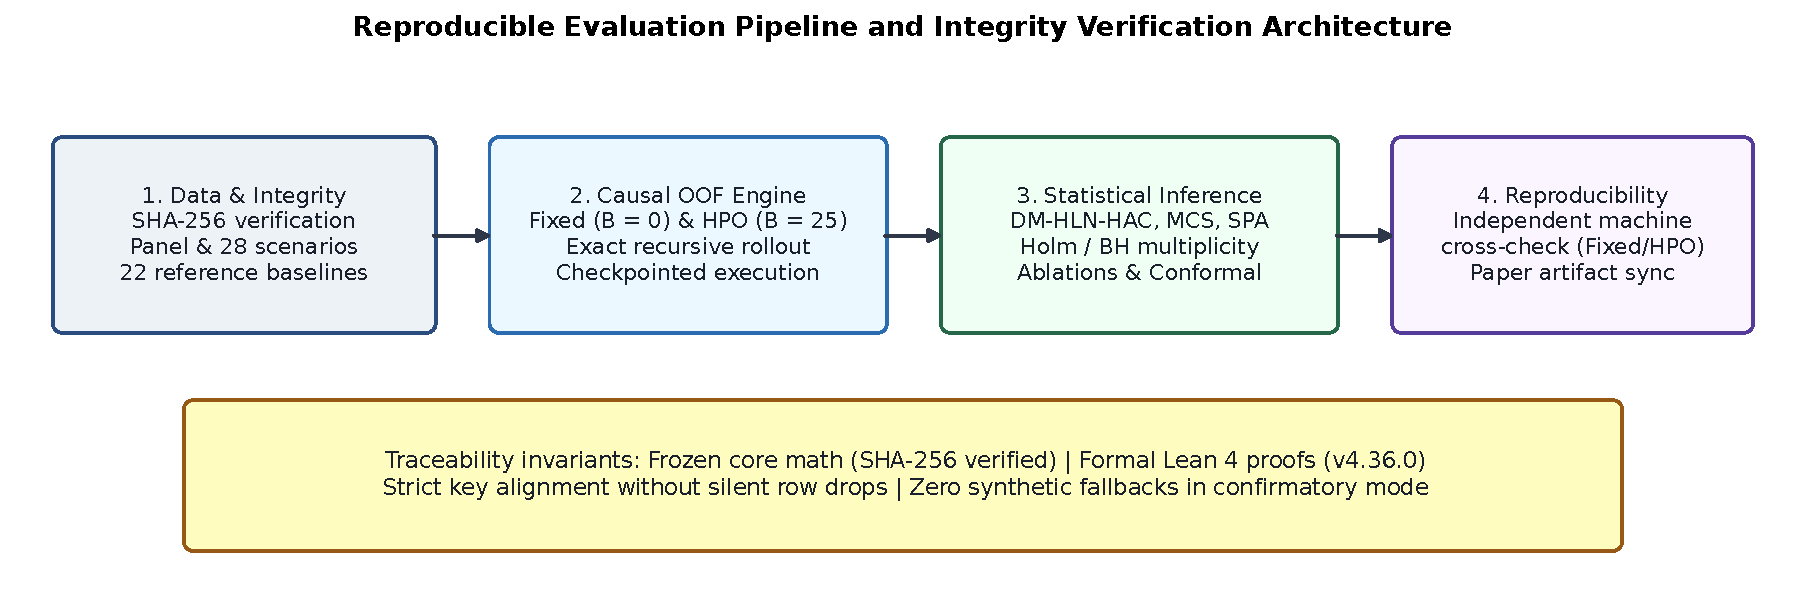
\includegraphics[width=0.95\textwidth]{figures/fig_pipeline_reproduccion.pdf}
\caption{Arquitectura de ejecución resumible y verificación de integridad de datos y resultados.}
\label{fig:sup_pipeline}
\end{figure}

\FloatBarrier
\section{Análisis exploratorio complementario y diagramas metodológicos}\label{sup:figuras}

Esta sección reúne las figuras exploratorias complementarias de la cohorte (Figuras~\ref{fig:sup_cohorte_mapa}--\ref{fig:sup_est_clima}) y los diagramas detallados de despliegue multihorizonte, estructura de la pérdida de Huber y validación cruzada causal anidada (Figuras~\ref{fig:sup_despliegue}--\ref{fig:sup_validacion}).

\begin{figure}[!htbp]
\centering
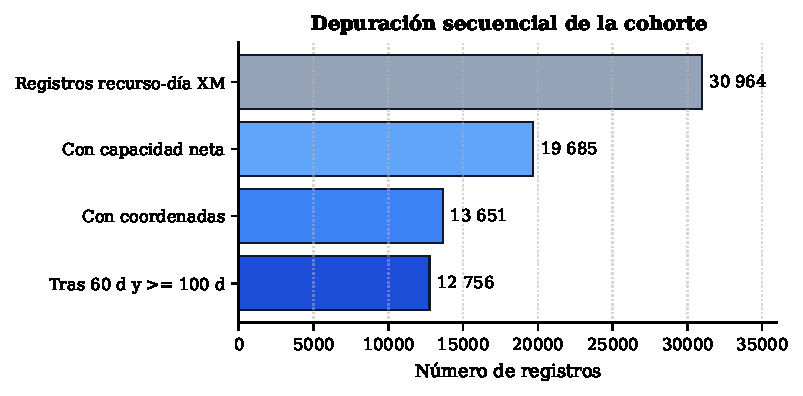
\includegraphics[width=0.84\textwidth]{figures/eda_flujo_cohorte.pdf}\\[0.5em]
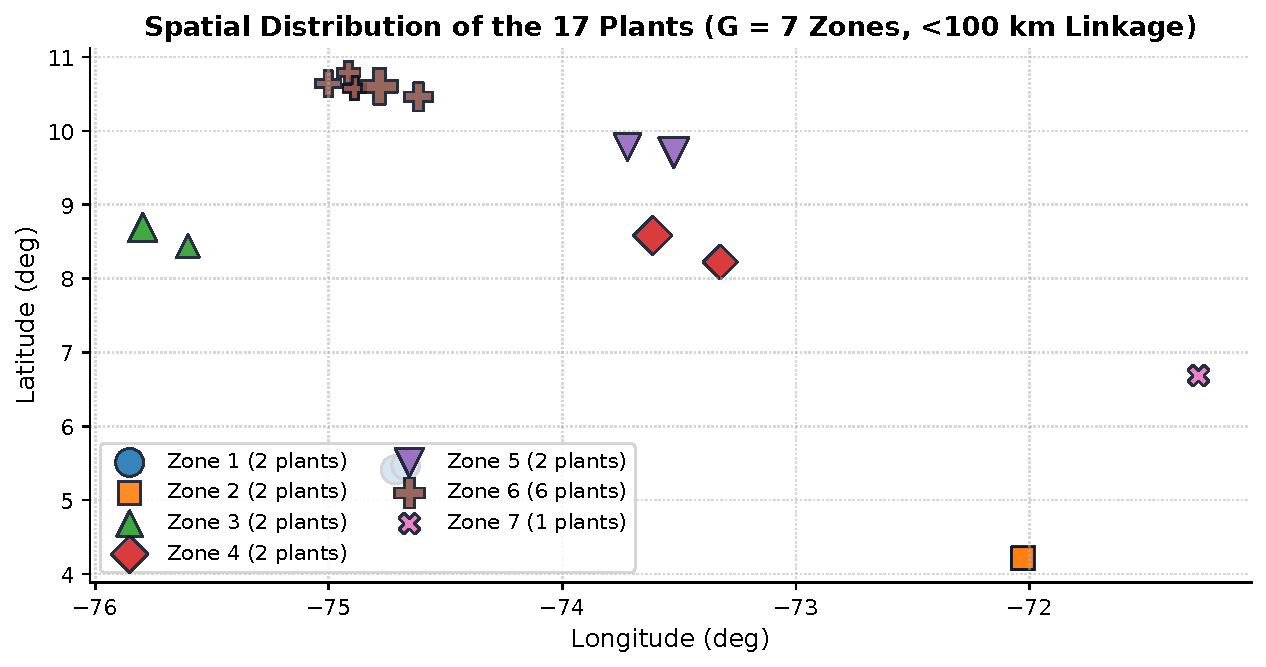
\includegraphics[width=0.84\textwidth]{figures/eda_mapa_plantas.pdf}
\caption{Depuración cuantitativa de la cohorte ($30\,964 \to 12\,756$ registros planta--día en $17$ centrales; arriba) y distribución geográfica en $G=7$ zonas espaciales por enlace simple a $<100\text{ km}$ (abajo).}
\label{fig:sup_cohorte_mapa}
\end{figure}

\begin{figure}[!htbp]
\centering
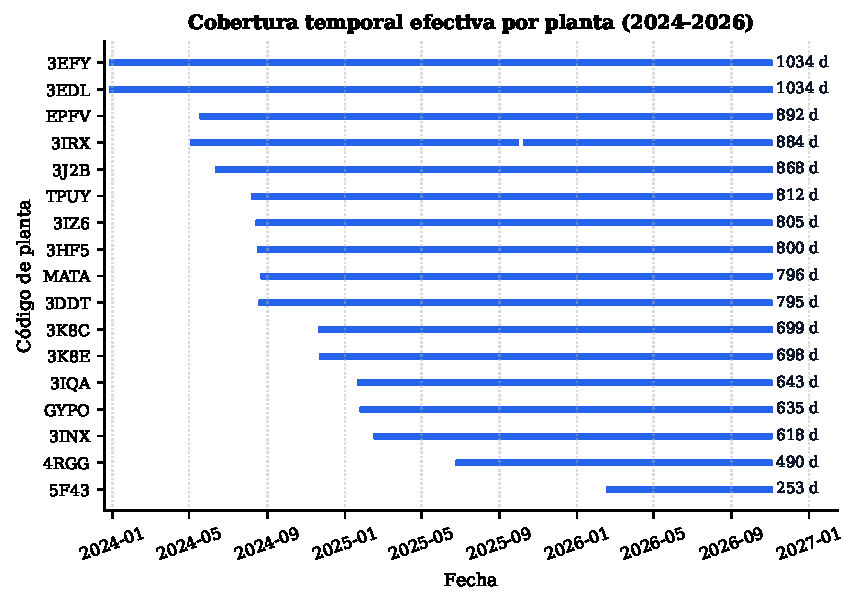
\includegraphics[width=0.90\textwidth]{figures/eda_cobertura_temporal.pdf}\\[0.5em]
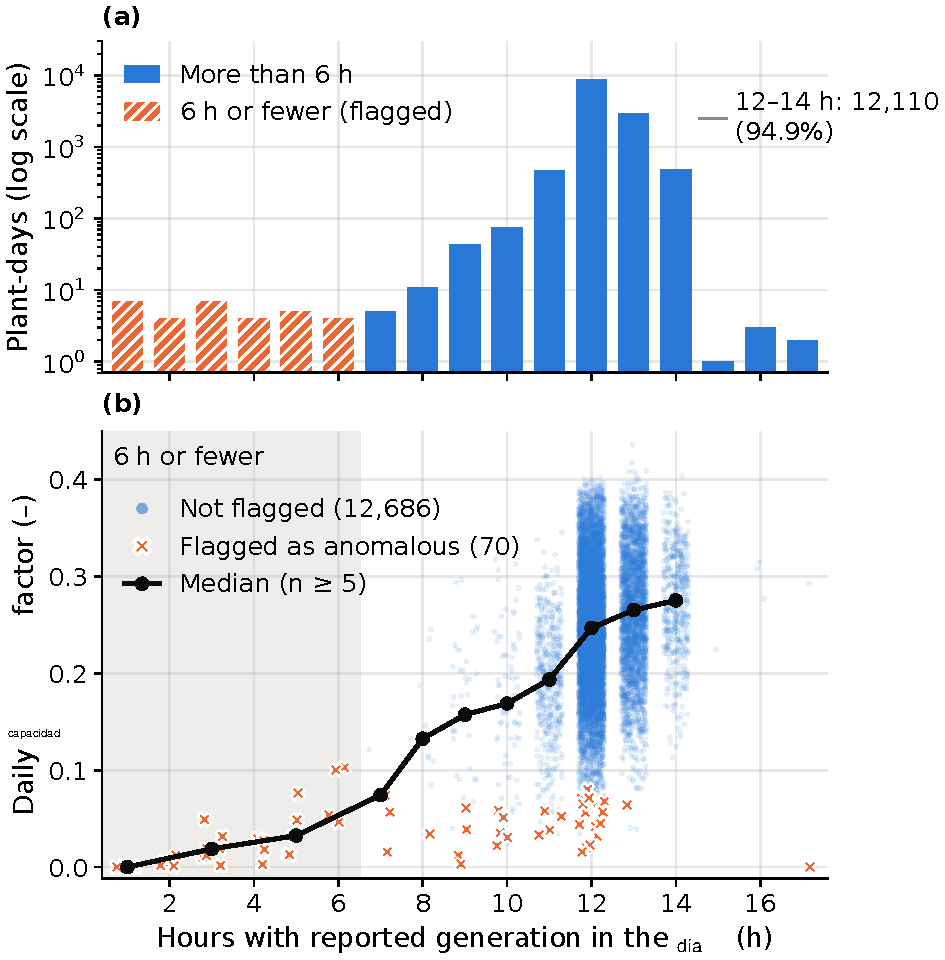
\includegraphics[width=0.90\textwidth]{figures/eda_horas_y_anomalos.pdf}
\caption{Cobertura temporal escalonada por planta ($251$ a $1\,032$ días útiles; arriba) y distribución de horas reportadas por XM mostrando los $31$ registros incompletos excluidos ($\le 6\text{ h}$; abajo).}
\label{fig:sup_cob_horas}
\end{figure}

\begin{figure}[!htbp]
\centering
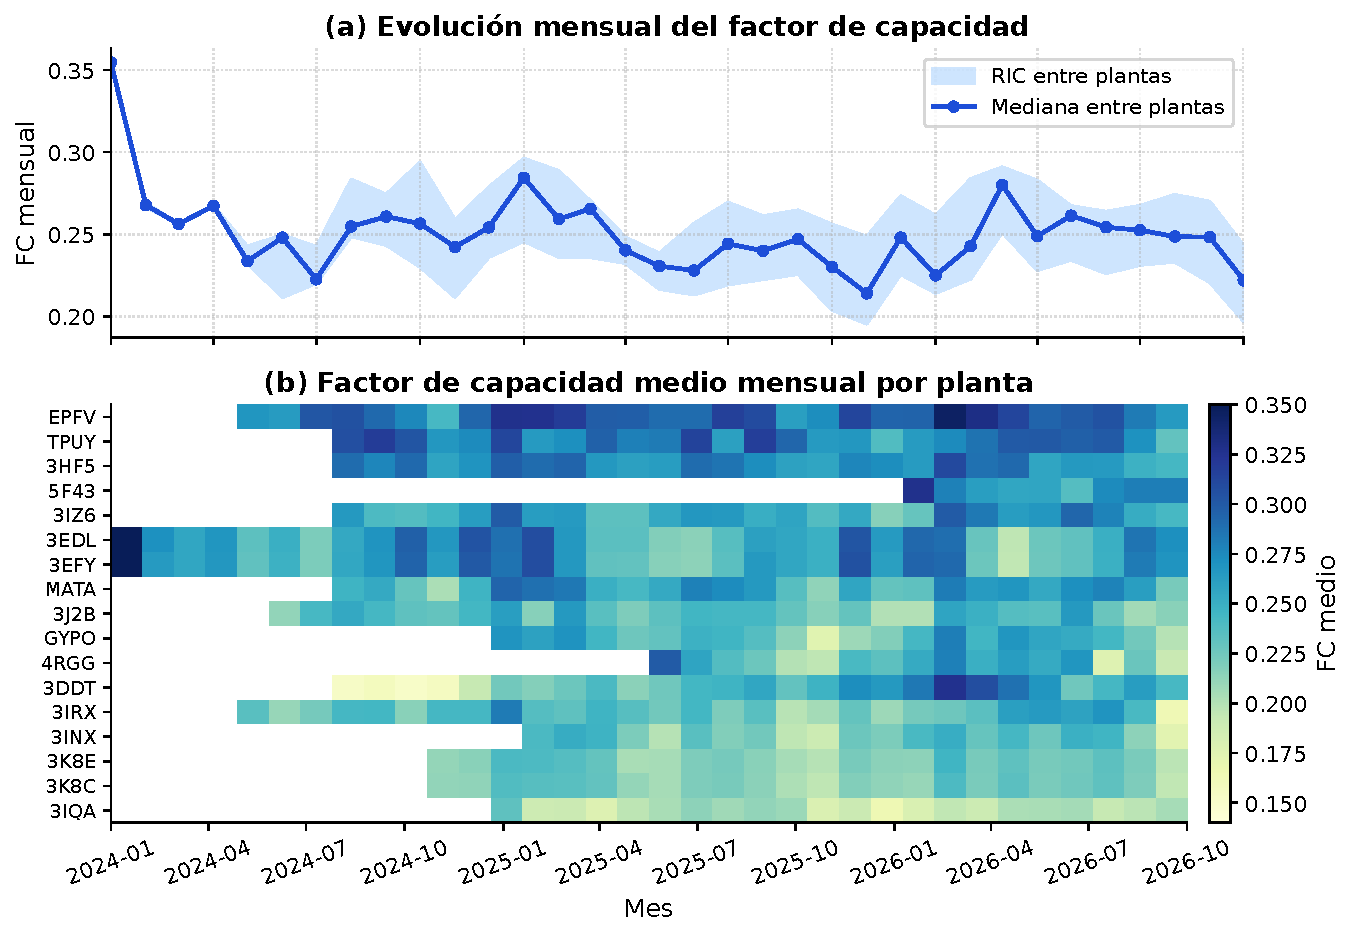
\includegraphics[width=0.90\textwidth]{figures/eda_estacionalidad.pdf}\\[0.5em]
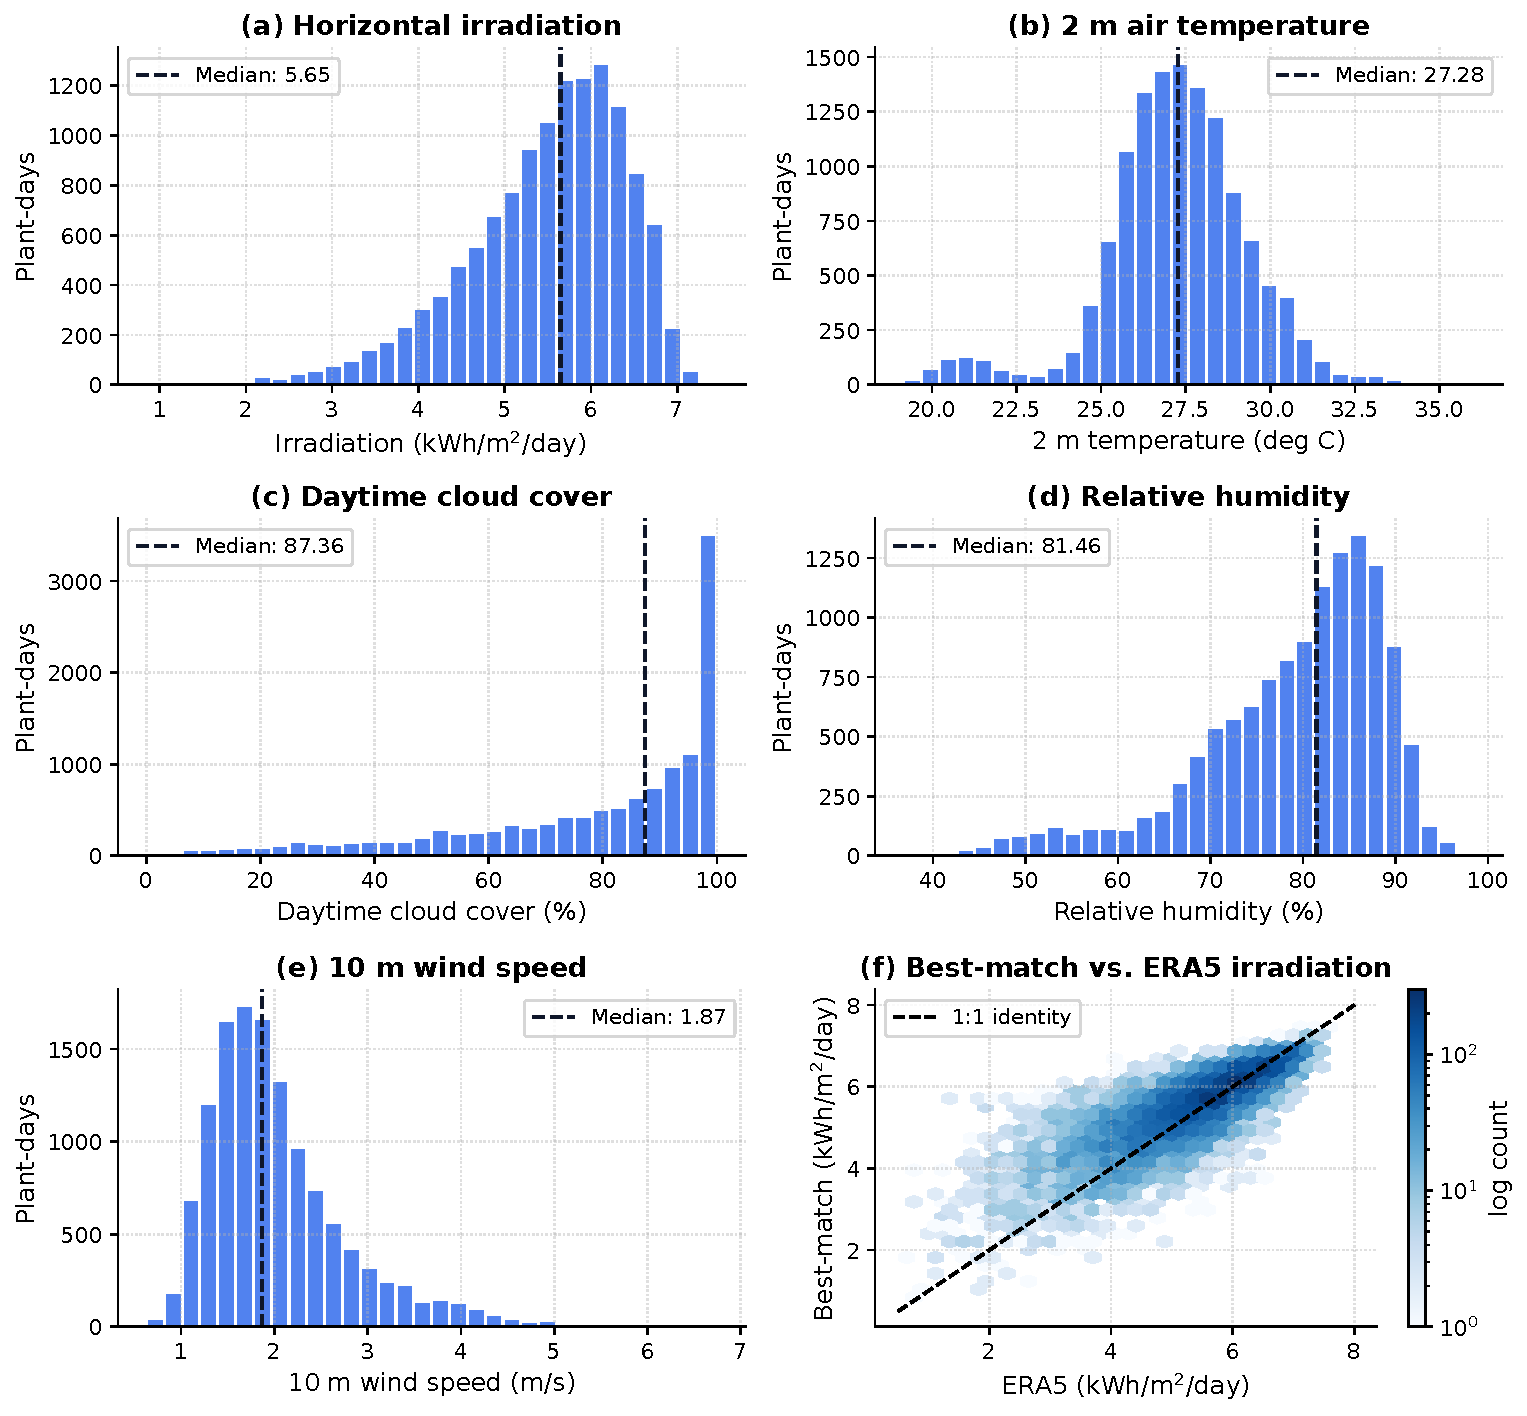
\includegraphics[width=0.90\textwidth]{figures/eda_clima.pdf}
\caption{Estacionalidad mensual del factor de capacidad (arriba) y distribución de las cinco variables meteorológicas pronosticadas sobre la cohorte (abajo).}
\label{fig:sup_est_clima}
\end{figure}

\begin{figure}[!htbp]
\centering
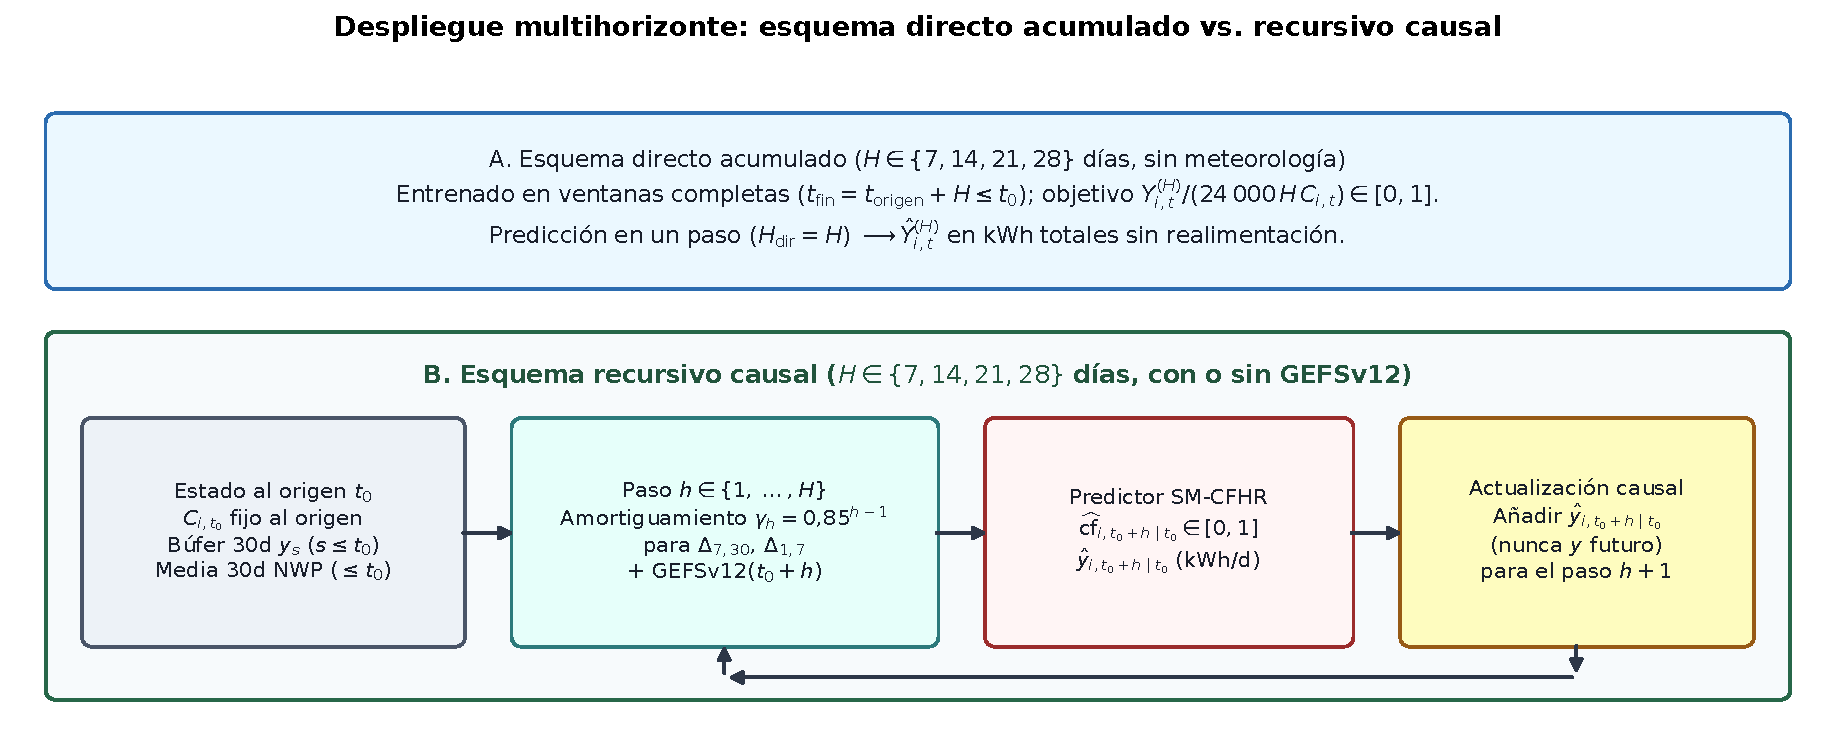
\includegraphics[width=0.95\textwidth]{figures/fig_despliegue_multihorizonte.pdf}
\caption{Comparación estructural entre el esquema directo acumulado ($H_{\mathrm{dir}}=H$, sin realimentación) y el despliegue recursivo multihorizonte con actualización causal mediante predicciones propias.}
\label{fig:sup_despliegue}
\end{figure}

\begin{figure}[!htbp]
\centering
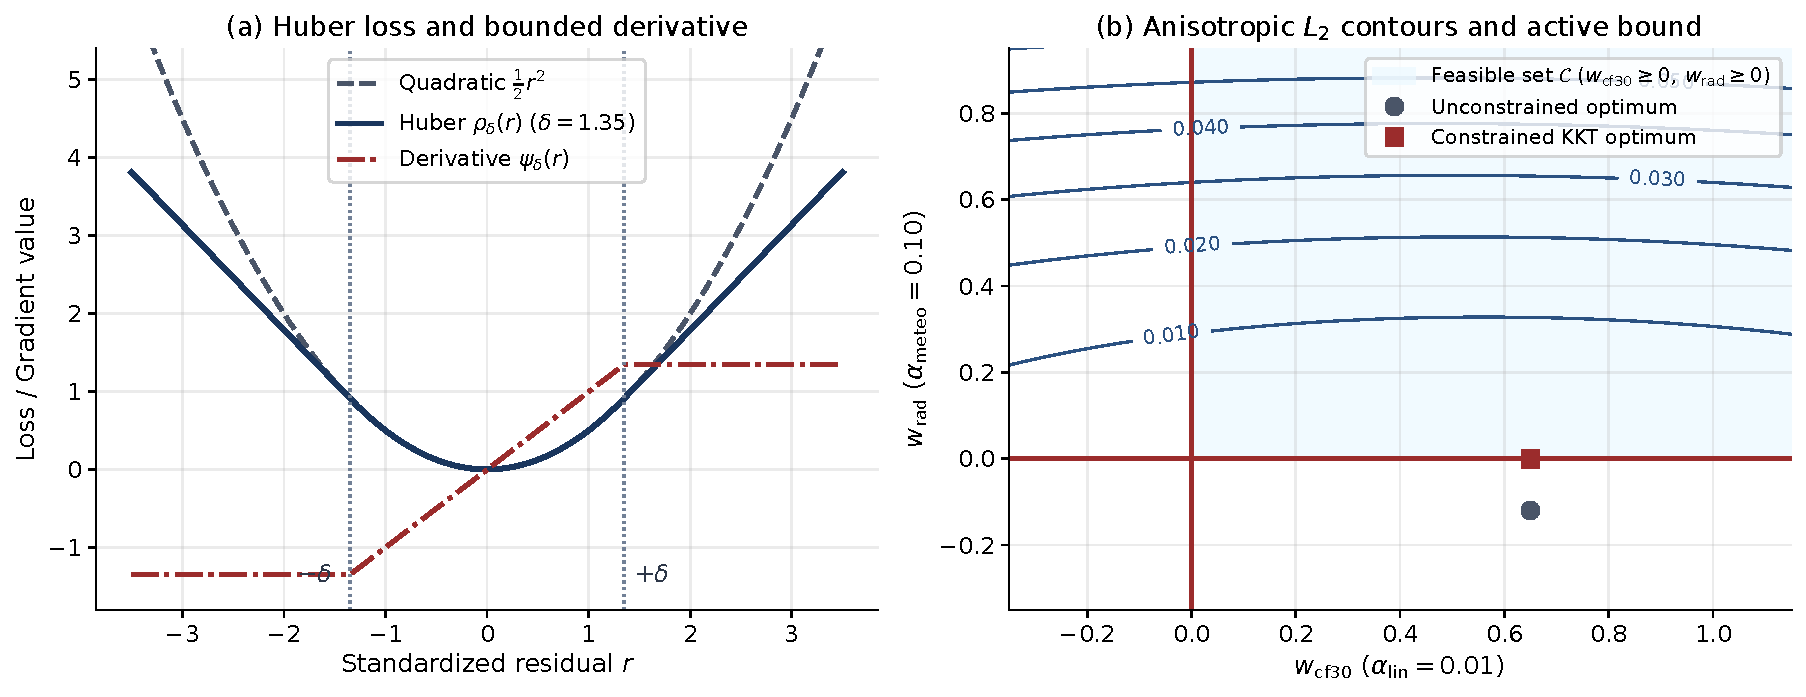
\includegraphics[width=0.95\textwidth]{figures/fig_huber_estructura.pdf}
\caption{Estructura analítica de SM-CFHR: pérdida de Huber $\rho_\delta(r)$ y derivada acotada $\psi_\delta(r)$ para $\delta = 1{,}35$ (izquierda), y curvas de nivel de la penalización $L_2$ anisotrópica con cota activa sobre $\mathcal{C}$ (derecha).}
\label{fig:sup_huber}
\end{figure}

\begin{figure}[!htbp]
\centering
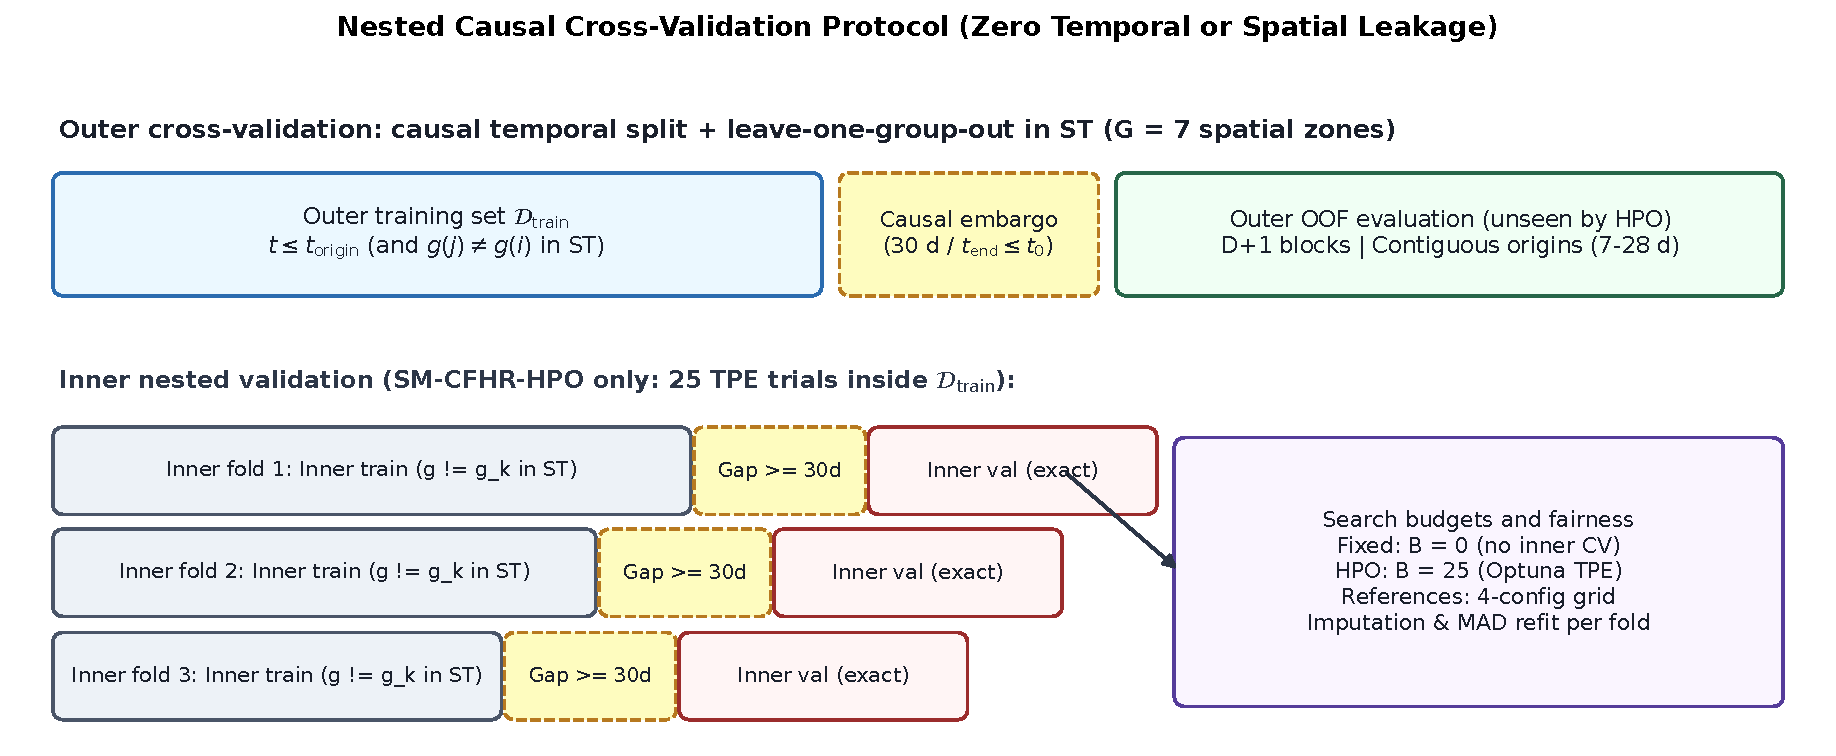
\includegraphics[width=0.95\textwidth]{figures/fig_validacion_anidada.pdf}
\caption{Esquema de validación cruzada causal anidada: separación temporal y espacial externa (\textit{leave-one-group-out} en ET) con brecha de embargo causal de $30$ días y validación interna de $3$ particiones para Optuna TPE.}
\label{fig:sup_validacion}
\end{figure}

\let\oldthebibliography\thebibliography
\renewcommand{\thebibliography}[1]{\oldthebibliography{#1}\small\setlength{\itemsep}{1pt plus 0.5pt minus 0.5pt}\setlength{\parskip}{0pt}}
\bibliographystyle{plain}
\bibliography{bibliography/bibliography}

\end{document}
